\chapter{Desenvolvimento e Produto}
\label{Produto}

Este capítulo deve mostrar as ferramentas utilizadas, as dificuldades encontradas ao desenvolver o produto e, também, imagens do produto desenvolvido.

\section{O que devo escrever aqui?}
Bem, quando você iniciou seu trabalho, você tinha um problema claro a resolver.
Você pesquisou a respeito do seu problema e também a respeito de ferramentas, tecnologias e outros recursos que poderiam ajudá-lo a resolver seu problema. No método você estabeleceu os passos usados para resolver o problema. Agora é hora de mostrar em detalhes que você alcançou os objetivos definidos na \nameref{Introducao}.

Você pode utilizar alguns comandos específicos para referenciar seus elementos:
\begin{itemize}
    \item \textbf{refFig:} Para referências de imagens que se iniciem com a palavra "Figura". Esta referência já escreve a palavra "Figura". Ex.: \refFig{fig:example}
    \item \textbf{refTab:} Para referências de tabelas que se iniciem com a palavra "Tabela". Esta referência já escreve a palavra "Tabela". Ex.: \refTab{tab:longtable}
    \item \textbf{refTabs:} Para referências de múltiplas tabelas. Esta referência escreve "Tabelas \# a \#". Ex.: \refTabs{tab:longtable}{tab:longtable}
    \item \textbf{refCap:} Para referências de capítulos que se iniciem com a palavra "Capítulo". Esta referência já escreve a palavra "Capítulo". Ex.: \refCap{Analise}. \nameref{Analise} também é outra forma de referenciar, caso necessite mostrar o título do capítulo.
    \item \textbf{refApendice:} Para referências de apêndices que se iniciem com a palavra "Apêndice". Esta referência já escreve a palavra "Apêndice". Ex.: \refApendice{apendice}
\end{itemize}

Por fim, na \refTab{tab:longtable}, temos um exemplo de longtable para referência.

\begin{longtable}[H]{|p{15em}|p{20em}|}
\caption{Exemplo de longtable} \label{tab:longtable} \\
\hline
\rowcolor[HTML]{eeeeee} \textbf{Cabeçalho 1}
& \textbf{Cabeçalho 2}
\\ \hline
\endfirsthead
         
\cellcolor[HTML]{eeeeee}Célula colorida
& 
Célula sem cor
\\ \hline 
         
\rowcolor[HTML]{eeeeee}\multicolumn{2}{|c|}{Linha colorida mesclada}
\\ \hline 

\rowcolor[HTML]{eeeeee}
Célula colorida sem negrito
& Célula colorida sem negrito
\\ \hline 
         
Conteúdo
& 
\\ \hline 

 &Conteúdo
\\ \hline

Conteúdo
& Conteúdo \\ \hline
\end{longtable}

% [H] para forçar posicionamento da imagem
\begin{figure}[H]
    \centering
    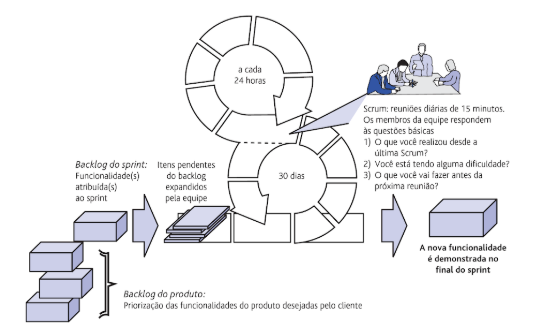
\includegraphics[width=1\linewidth]{img/scrum.PNG}
    \caption{Exemplo de Imagem}
    \label{fig:example}
\end{figure}